\documentclass{standalone}

\usepackage{tikz}
\usepackage{pgfplots}
\begin{document}
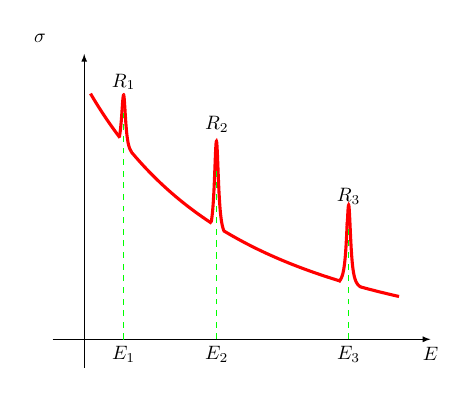
\begin{tikzpicture}[scale=0.7] % Reduce la escala al 70%
    \begin{axis}[
        xmin=-1, xmax=11, % Establece el rango del eje x
        ymin=-0.1, ymax=1, % Ajusta el rango para el eje y
        smooth,
        samples=100,
        tick style={draw=none}, % Oculta los tics de los ejes
        xtick=\empty, % Elimina los números del eje x
        ytick=\empty, % Elimina los números del eje y
        axis lines=middle,
        axis line style={-latex}, % Flechas en los ejes
        xlabel={$E$},
        ylabel={$\sigma$},
        xlabel style={at={(axis description cs:1.0,0)}, anchor=south}, % Debajo de la flecha del eje x
        ylabel style={at={(axis description cs:0,1.05)}, anchor=east} % A la izquierda de la flecha del eje y
    ]

    % Primeras curvas
    \addplot[red, ultra thick, domain=0.2:1.136] {100/(x+10)^2-0.1};
    \addplot[red, ultra thick, domain=1.49:4.05] {100/(x+10)^2-0.1};
    \addplot[red, ultra thick, domain=4.415:8.15] {100/(x+10)^2-0.1};
    \addplot[red, ultra thick, domain=8.795: 10] {100/(x+10)^2-0.1};

    % Lorentzianas ajustadas
    % Entre 1 y 1.5
    \addplot[red, ultra thick, domain=1.115:1.25] {0.2 / (1 + ((x-1.25)/0.08)^2) + (100/(1.5+10)^2-0.1)};

    \addplot[red, ultra thick, domain=1.248:1.5] {0.22 / (1 + ((x-1.25)/0.08)^2) + (100/(1.5+10)^2-0.119)};
    
    % Entre 4 y 5
    \addplot[red, ultra thick, domain=4.035:4.435] {0.35 / (1 + ((x-4.2)/0.08)^2) + (100/(5+10)^2-0.1)};
    
    % Entre 8 y 8.8
    \addplot[red,ultra thick, domain=8.09:8.355] {0.3 / (1 + ((x-8.4)/0.08)^2) + (100/(8.8+10)^2-0.1)};
    \addplot[red,ultra thick, domain=8.355:8.8] {0.3 / (1 + ((x-8.4)/0.08)^2) + (100/(8.8+10)^2-0.112)};

    % Líneas verticales dashed verdes
    \addplot[green, dashed] coordinates {(1.25,0) (1.25,0.8)};
    \addplot[green, dashed] coordinates {(4.21,0) (4.21,0.6)};
    \addplot[green, dashed] coordinates {(8.4,0) (8.4,0.4)};

    \node[below] at(axis cs: 1.25,0){$E_1$};
    \node[below] at(axis cs: 4.21,0){$E_2$};
    \node[below] at(axis cs: 8.4,0){$E_3$};

    \node[above] at(axis cs: 1.25,0.85){$R_1$};
    \node[above] at(axis cs: 4.21,0.7){$R_2$};
    \node[above] at(axis cs: 8.4,0.45){$R_3$};
    \end{axis}
\end{tikzpicture}
\end{document}
